\documentclass[a4paper, 12pt]{book}
% preamble.tex

\usepackage[utf8]{inputenc}
\usepackage[T1]{fontenc}
\usepackage[english]{babel} % Ho cambiato in italian, supponendo che la maggior parte del testo sia in italiano
\usepackage{amsmath}
\usepackage{amssymb}
\usepackage{graphicx}
\usepackage{hyperref}
\usepackage{geometry}
\usepackage{fontspec} % Utile per Xetex/LuaLaTeX ma mantenuto
\usepackage{booktabs}
\usepackage{amsthm}
\usepackage{enumitem}
\usepackage{caption}
\usepackage{thmtools}
\usepackage{standalone} % Già presente nel tuo elenco
\usepackage{tkz-euclide}
\usepackage{graphicx}
\usepackage[T1]{fontenc}
\usepackage{wesa}

% --- PACCHETTI AGGIUNTI PER LA FORMATTAZIONE ---
\usepackage{parskip}  % Aggiunge spazio tra i paragrafi (stile "blocco")
\usepackage{fancyhdr} % Per intestazioni e piè di pagina personalizzati

% --- IMPOSTAZIONI GEOMETRIA E FONT ---
\geometry{a4paper, margin=1in}

% Configura lo stile 'plain' (usato da \maketitle e \tableofcontents)
% per essere coerente con il piè di pagina
\fancypagestyle{plain}{
    \fancyhf{} % Pulisce
    \cfoot{\thepage} % Mette solo il numero di pagina
    \renewcommand{\headrulewidth}{0pt} % Niente linea su queste pagine
}

% Configurazione Header/Footer per le altre pagine
\pagestyle{fancy}
\fancyhead{} % Pulisce l'intestazione
\fancyfoot{} % Pulisce il piè di pagina
\fancyhead[L]{\nouppercase{\rightmark}} % Nome Sezione a sinistra (o Chapter)
\fancyhead[R]{\nouppercase{\leftmark}}  % Nome Capitolo a destra (o Sezione)
\fancyfoot[C]{\thepage} % Numero di pagina al centro
\renewcommand{\headrulewidth}{0.4pt}
\renewcommand{\footrulewidth}{0pt}


% --- DEFINIZIONI TEOREMI ---
% (Questa parte è cruciale per la tua struttura)
\newtheoremstyle{mythmstyle}%
    {}%
    {}%
    {\itshape}%
    {}%
    {\bfseries}%
    {}%
    { }%
    {\thmname{#1}\thmnumber{ #2}%
    \thmnote{: #3\addcontentsline{toc}{subsubsection}{{\itshape#1}: #3}}. }

% 2. Imposta questo stile come quello ATTUALE
\theoremstyle{mythmstyle}

\newtheorem{theorem}{Th}[section]
\newtheorem{definition}{Def}[section]
\newtheorem{proposition}{Prop}[section]
\newtheorem{corollary}{Cor}[section]
\newtheorem{algorithm}{Alg}[section]
\newtheorem{lemma}{Lemma}[section]
\newtheorem*{remark}{Rem}

% Definizioni utili per il Main file
\newcommand{\inputlesson}[1]{\clearpage\input{#1}\clearpage} % Comando per input lezione
\usepackage[x11names]{xcolor}
\usepackage{tikz}
\usetikzlibrary{shapes,fit}
\usepackage{amsmath} % Required for align environment
\usepackage{caption} % Required for \captionof outside float environments


\begin{document}
\setcounter{chapter}{7}
\chapter{Lesson 2-12-2025}
\section[Mathematical representation of OFDM]{Mathematical representation of OFDM, noise of a subcarrier; terminology used by the book; pulse shaping for OFDM}

Given that the symbols we're generating and want to transmit are $\mathrm{x}[k]$, we have that after IDFT and cyclic prefix, the OFDM waves will be

\begin{align}
    \bar{x}[n] = \frac{1}{K} \sum_{k=0}^{K-1} \mathrm{x}[k] e^{j \frac{2\pi}{K} nk} \quad n = -L, \dots, K-1 \tag{2.211}
\end{align}

\begin{itemize}[label=\textcolor{red}{\small\faSquare}]
    \item \textbf{Transmitted samples after the IDFT and cyclic prefix addition}
    \begin{align*}
        \bar{x}[n] = \frac{1}{K} \sum_{k=0}^{K-1} \mathrm{x}[k] e^{j \frac{2\pi}{K} nk} \quad n = -L, \dots, K-1
    \end{align*}

    \item \textbf{Received signal after discarding the cyclic prefix (first L samples)}

    \noindent
    \begin{minipage}[t]{0.45\textwidth}
        \begin{align*}
            y[n] &= \sqrt{G} \sum_{\ell=0}^{L} h[\ell] \bar{x}[n-\ell] \\
            &= \sqrt{G} \sum_{\ell=0}^{L} h[\ell] x[(n-\ell)_K] \quad n=0, \dots, K-1
        \end{align*}
        \textcolor{orange}{\small Looks like a circular convolution \\ between length K signals \\ (channel zero padded)}
    \end{minipage}%
    \begin{minipage}[t]{0.1\textwidth}
        \centering
        \vspace{1.5cm}
        \textcolor{orange}{\Huge $\Rightarrow$}
    \end{minipage}%
    \begin{minipage}[t]{0.45\textwidth}
        \vspace{0.5cm}
        \textcolor{purple}{\small (now including noise)}
        \begin{align*}
            \mathrm{y}[k] = \sqrt{G} \mathrm{h}[k]\mathrm{x}[k] + \mathrm{v}[k]
        \end{align*}
        \textcolor{orange}{\small Simple equalization} \\
        \raggedleft
        \small $\swarrow$ \textcolor{orange}{\small Noise remains IID and $\sim \mathcal{N}_{\mathbb{C}}(0, N_0)$}
    \end{minipage}

    \vspace{1em}
    \begin{center}
        \colorbox{cyan!15}{
            \begin{minipage}{0.3\textwidth}
                \centering
                \small \textbf{Per-subcarrier noise}
                \[
                \frac{N_0}{G} \frac{1}{|h[k]|^2}
                \]
            \end{minipage}
        }
    \end{center}
\end{itemize}

Professor never used the \textit{circular convolution}.
We sum the noise which is IID and Gaussian.

\vspace{1cm}
\noindent\textbf{\large Note:} \\
\textsf{Vedi: ex 2.22, 2.23 (esercizi esame molto simili a quelli del libro + vedi moodle)}
We can see that each \textbf{subcarrier has a noise variance} of
\begin{align}
    \frac{N_0}{G} \frac{1}{|h[k]|^2}. \tag{2.221}
\end{align}
This follow from the type of equalization we're performing (specifically by using (2.219) to find the noise covariance by considering $\hat{\mathrm{x}}[k] \hat{\mathrm{x}}^*[k]$ for symbols $x_k \equiv \mathrm{x}[k] = 0$, s to only consider the noise),

\vspace{0.5cm}

\noindent
\fcolorbox{cyan}{white}{
    \begin{minipage}{0.95\linewidth}
        \vspace{0.2cm}
        \textcolor{cyan}{\faPen\ \textbf{My explanation}}
        
        At a certain point we get that (with reference to A signal processing perspective (pp. 57-130), p. 50):
        
        \begin{align*}
            y[n] = \sum_{k=0}^{K-1} x_k h[k] e^{j \frac{2\pi}{K}kn},
        \end{align*}
        
        which is the IDFT of $x_k h[k]$! We know that a zero forcing equalizer $W$ is such that in the frequency domain, we'll have
        
        \begin{align*}
            W^*(z) \cdot H(z) = z^{-\Delta}.
        \end{align*}
        
        What we see here is that we have a \textit{dummy frequency domain} which sees the multiplication of $x_k$ and $h[k]$: this will allow us to say that if we choose
        
        \begin{align*}
            x_k = \frac{1}{K h[k]} \mathrm{DFT}[y[n] \mid k],
        \end{align*}
        
        the relation will be satisfied with $\Delta = 0$: in this sense, what we previously found can be considered a ZF equalizer.
        
        If we then were to also add the channel gain $\sqrt{G}$ into the mix and we defined $\hat{\mathrm{x}}[k] \equiv x_k$ and $\mathrm{y}[k] = \mathrm{DFT}[y \mid k]$, we have that the previous equation can be written just like in the book,
        
        \begin{align}
            \hat{\mathrm{x}}[k] = \frac{\mathrm{y}[k]}{\sqrt{G} h[k]} \quad k=0, \dots, K-1. \tag{2.219}
        \end{align}
        \vspace{0.1cm}
    \end{minipage}
}

\vspace{0.5cm}

If the channel is small for a certain $k$, the noise is increasing in the subcarriers. If the frequency response is small, we're paying this in increasing noise.

\noindent
\colorbox{teal!10}{
    \begin{minipage}{\linewidth}
        This is somehow tied to \texttt{\^{}d45a40}.
    \end{minipage}
}

\section*{Terminology:}

\begin{itemize}[label=\textcolor{red}{\small\faSquare}]
    \item Input to the IDFT are symbols
    \item Output of the IDFT are OFDM chips
    \item Interval between chips is T (would be the symbol period)
    \item Number of subcarriers is K, the dimension of the IDFT / DFT
    \item Collection of chips $\bar{x}[-L], \dots, \bar{x}[K-1]$ forms an OFDM symbol
    \item OFDM symbol period is (K+L)T
    \item Subcarrier spacing is the distance between adjacent subcarriers $\frac{1}{KT}$
    \item Effective pulse shape is usually a rectangular
    \item Edge subcarriers may be zero, leading to a spectral efficiency penalty
\end{itemize}

\vspace{0.5cm}

\noindent
\colorbox{teal!10}{
    \begin{minipage}{\linewidth}
        About chips: professor does not agree to this; \textit{chip} has to do with slicing.
    \end{minipage}
}

We have that $\mathrm{x}[k]$ are symbols, $\mathrm{z}[n]$ are chips.

The \textbf{interval between chips} is $T$.
The \textbf{number of subcarriers} is $K$; this is also the dimension of the IDFT/DFT.
The collection of chips $\bar{x}[-L], \dots, \bar{x}[K-1]$ forms an \textbf{OFDM symbol}: an OFDM symbol is $K+L$.

\vspace{0.5cm}
\begin{center}
    \begin{minipage}{0.5\linewidth}
        \centering
        \setlength{\fboxsep}{10pt}
        \begin{tabular}{@{}c@{}}
            \fbox{L}\fbox{\makebox[2cm]{K}} \\[-1ex]
            $\underbrace{\hspace{4.5cm}}_{K+L}$ \\
            \textcolor{blue!70}{\Huge $\swarrow$} \\
            \textcolor{blue!70}{\large Symbol period $(K+L)T$}
        \end{tabular}
    \end{minipage}
\end{center}
\vspace{0.5cm}

It's tricky to have to do with this: we do S/P, then DFT, then we add the cyclic prefix. We're adding some symbols: we'll need to go faster in order to keep up with the previous frequency.

\vspace{0.5cm}
\hrule
\vspace{0.5cm}

One way of choosing the pulse shape is to have a rectangular pulse of duration $KT$, giving that subcarriers will bring a signal of $KT \mathrm{sinc}(fKT)$.
In discrete frequency, the subcarriers are spaced of $1/K$, which, with a sampling period of $T$, gives that the $K$ subcarriers will \textbf{span a total bandwidth of $1/T$}.

The actual (non-ideal) signal will surely have a bandwidth larger than $1/T$, forcing us to set some of the outer carriers to $0$.
This can be done either by \textit{windowing}, aka by putting specific subcarriers to $\theta$ or by just applying a filter before transmission.

One thing which is typically done to improve the overall situation is to use raised cosines or similar signals.

$K \uparrow$ implies that the subcarriers are narrower and decay faster in frequencies. This term directly influences the containment of the signal in $1/T$.
Also, the higher this value, the more the subcarriers are susceptible to little changes.
(e.g.: if a subcarrier has a small phase shift, this causes more trouble if the symbols are tightly close).
As it's clear, $K$ also influences the resolution of the channel's frequency selectivity.

\vspace{0.5cm}

\noindent
\fcolorbox{gray!50}{white}{
    \begin{minipage}{0.95\linewidth}
        \vspace{0.2cm}
        \textcolor{gray}{\faLink\ \textbf{Comparisons}}
        
        The book makes some comparisons between OFDM and single-carrier techniques. I just skipped over that.
        If interested, see \textit{A signal processing perspective (pp. 57-130), p. 53}.
        \vspace{0.1cm}
    \end{minipage}
}

\vspace{0.5cm}

One last thing is that whenever the book (or this document) mentions \textit{OFDM resource elements}, we're referring to a specific OFDM symbol in time and a specific subcarrier in frequency, according to the figure:

\begin{figure}[h]
    \centering
    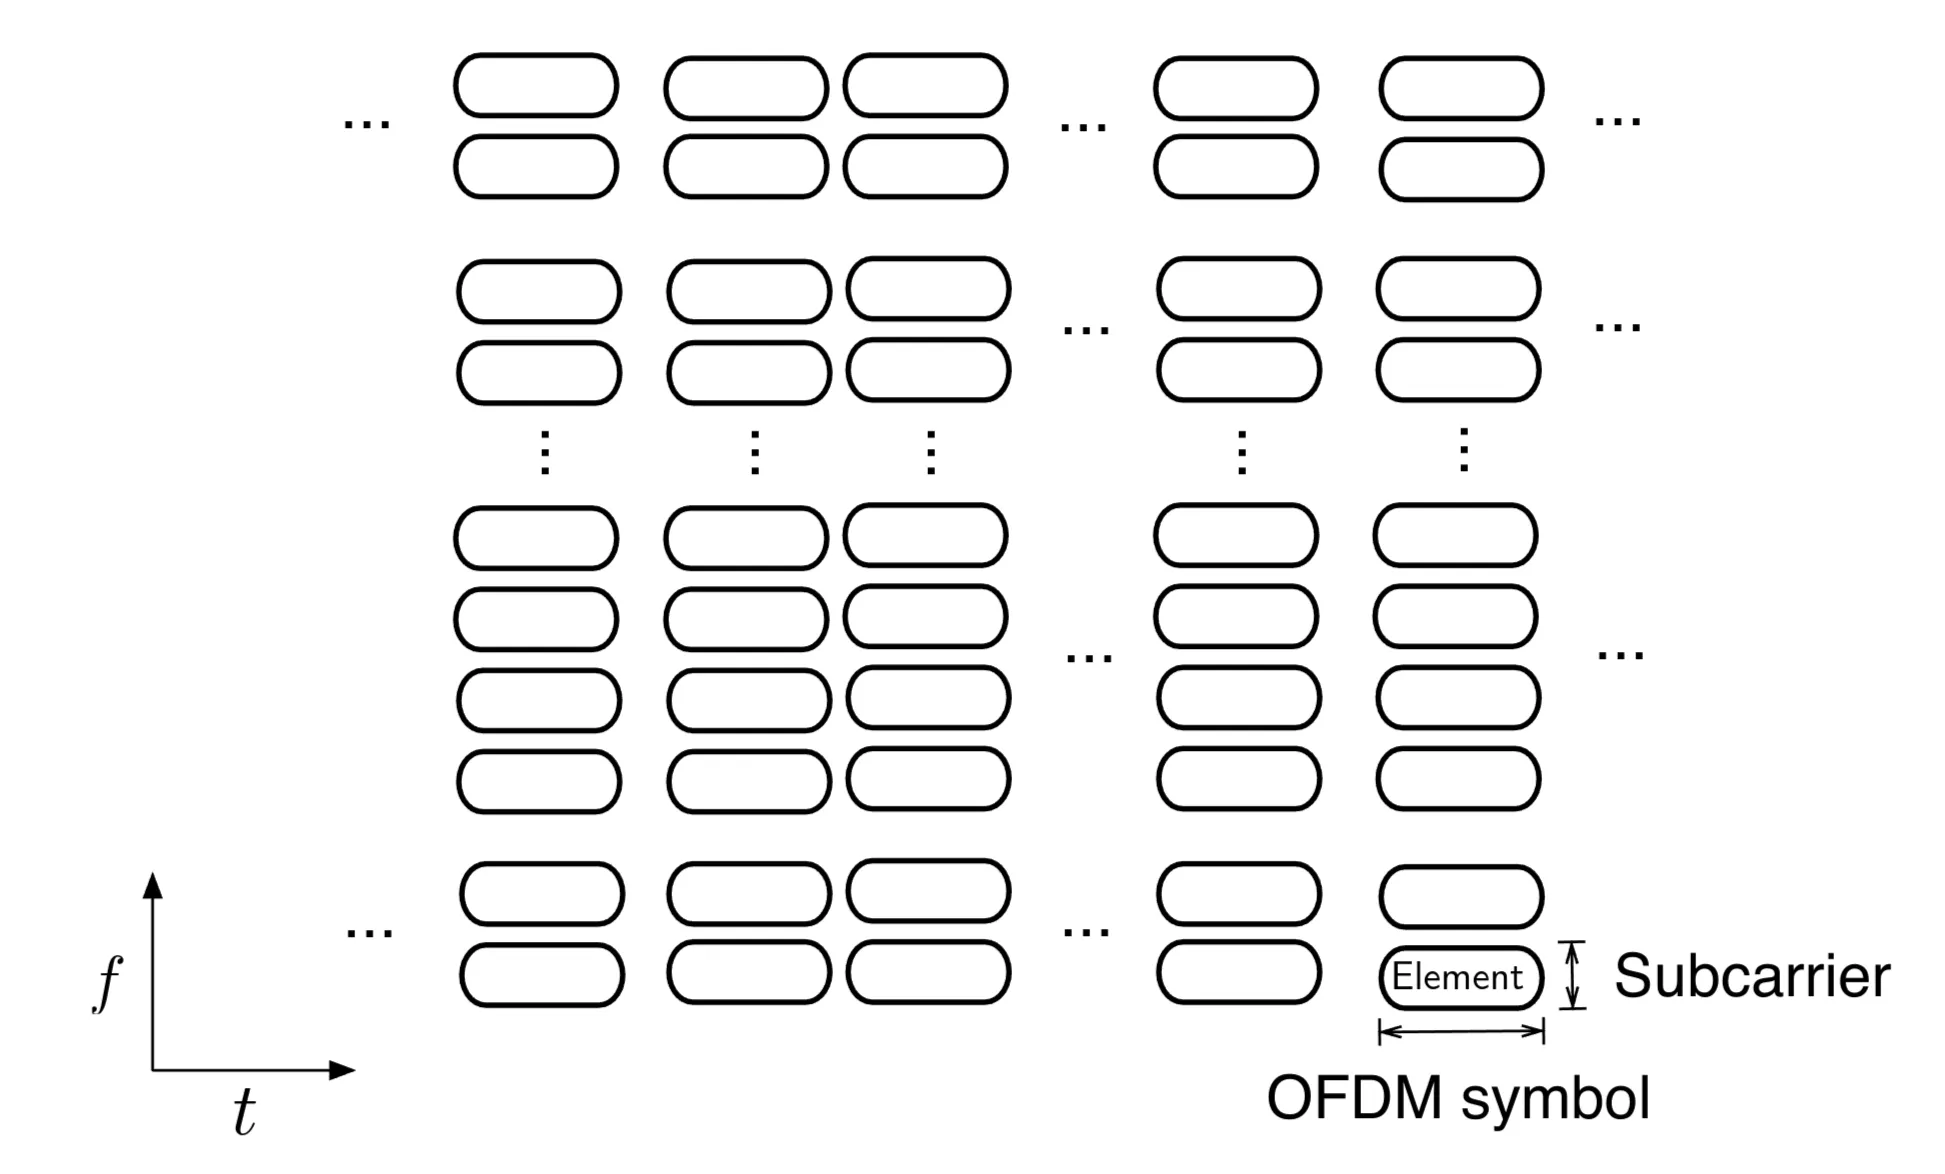
\includegraphics[width=0.6\textwidth]{Pictures/nome_immagine-004.png}
    \caption{OFDM resource elements representation}
\end{figure}

\section[Subcarrier spacing, spectral efficiency penalty]{Subcarrier spacing (+about the rectangular pulse shape of the signal), spectral efficiency penalty}

Subcarrier \textbf{spacing between adjacent carriers} is $1/KT$; this comes from the writing

\begin{align*}
    \exp \left( j \frac{2\pi}{K} kn \right) = \exp \left( j 2\pi \frac{k}{KT} nT \right).
\end{align*}

in which $k/KT$ is the frequency term and $nT$ is the time term.
The spacing in frequency between each subcarrier will thus be $1/KT$.

The pulse shape is usually rectangular. We'll eventually need to go back to the continuous time domain; if we go back, we'll see that we have $x[n]$ (the transmission will happen in continuous time, of course):

\begin{figure}[h]
    \centering
    % Inserire qui l'immagine del Trasmettitore con IDFT e Cyclic Prefix
    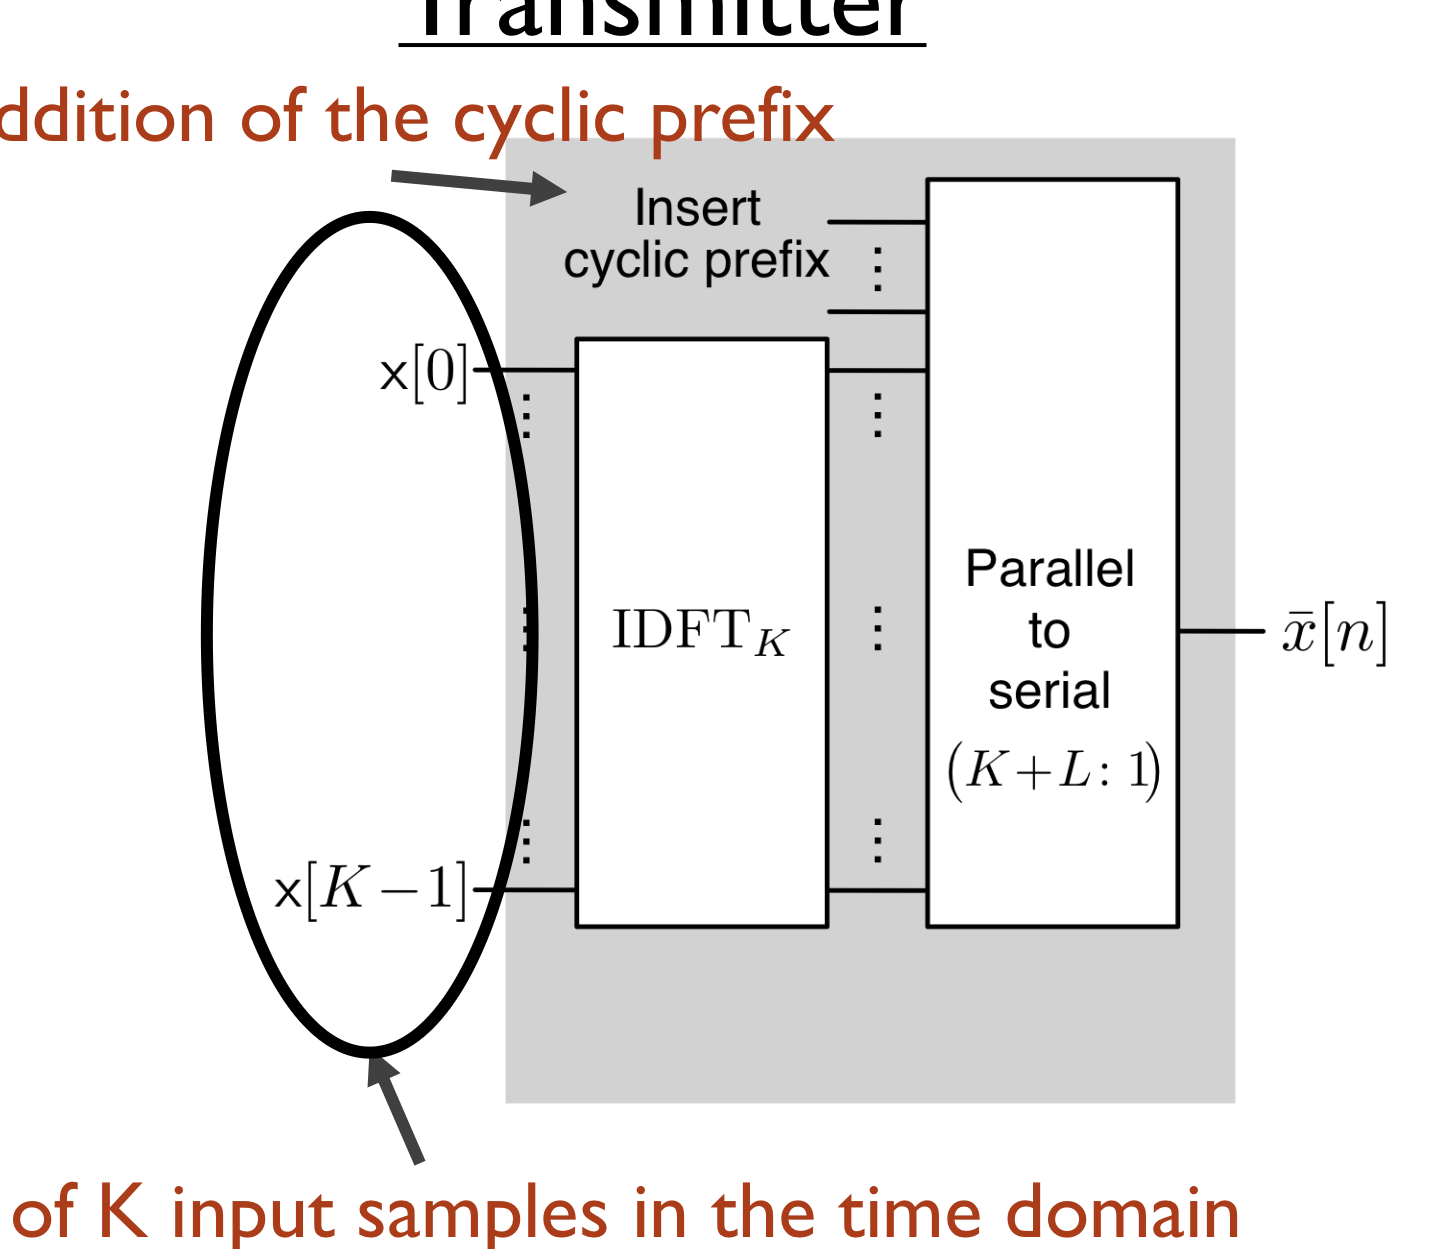
\includegraphics[width=0.4\textwidth]{Pictures/nome_immagine-005.png}
    \caption{Transmitter: addition of the cyclic prefix}
\end{figure}

We'll actually need to use a rect:

\begin{figure}[h]
    \centering
    % Inserire qui il grafico manuale del segnale rettangolare nel tempo (0 to KT)
    
\includegraphics[width=0.3\textwidth]{Pictures/image.png}
    \caption{Rectangular pulse of duration KT}
\end{figure}

This is pretty brutal, but we'll have a sinc in the frequency domain; all the multiples of $1/KT$ will be 0:

\begin{figure}[h]
    \centering
    % Inserire qui il grafico dei lobi Sinc sovrapposti in frequenza
    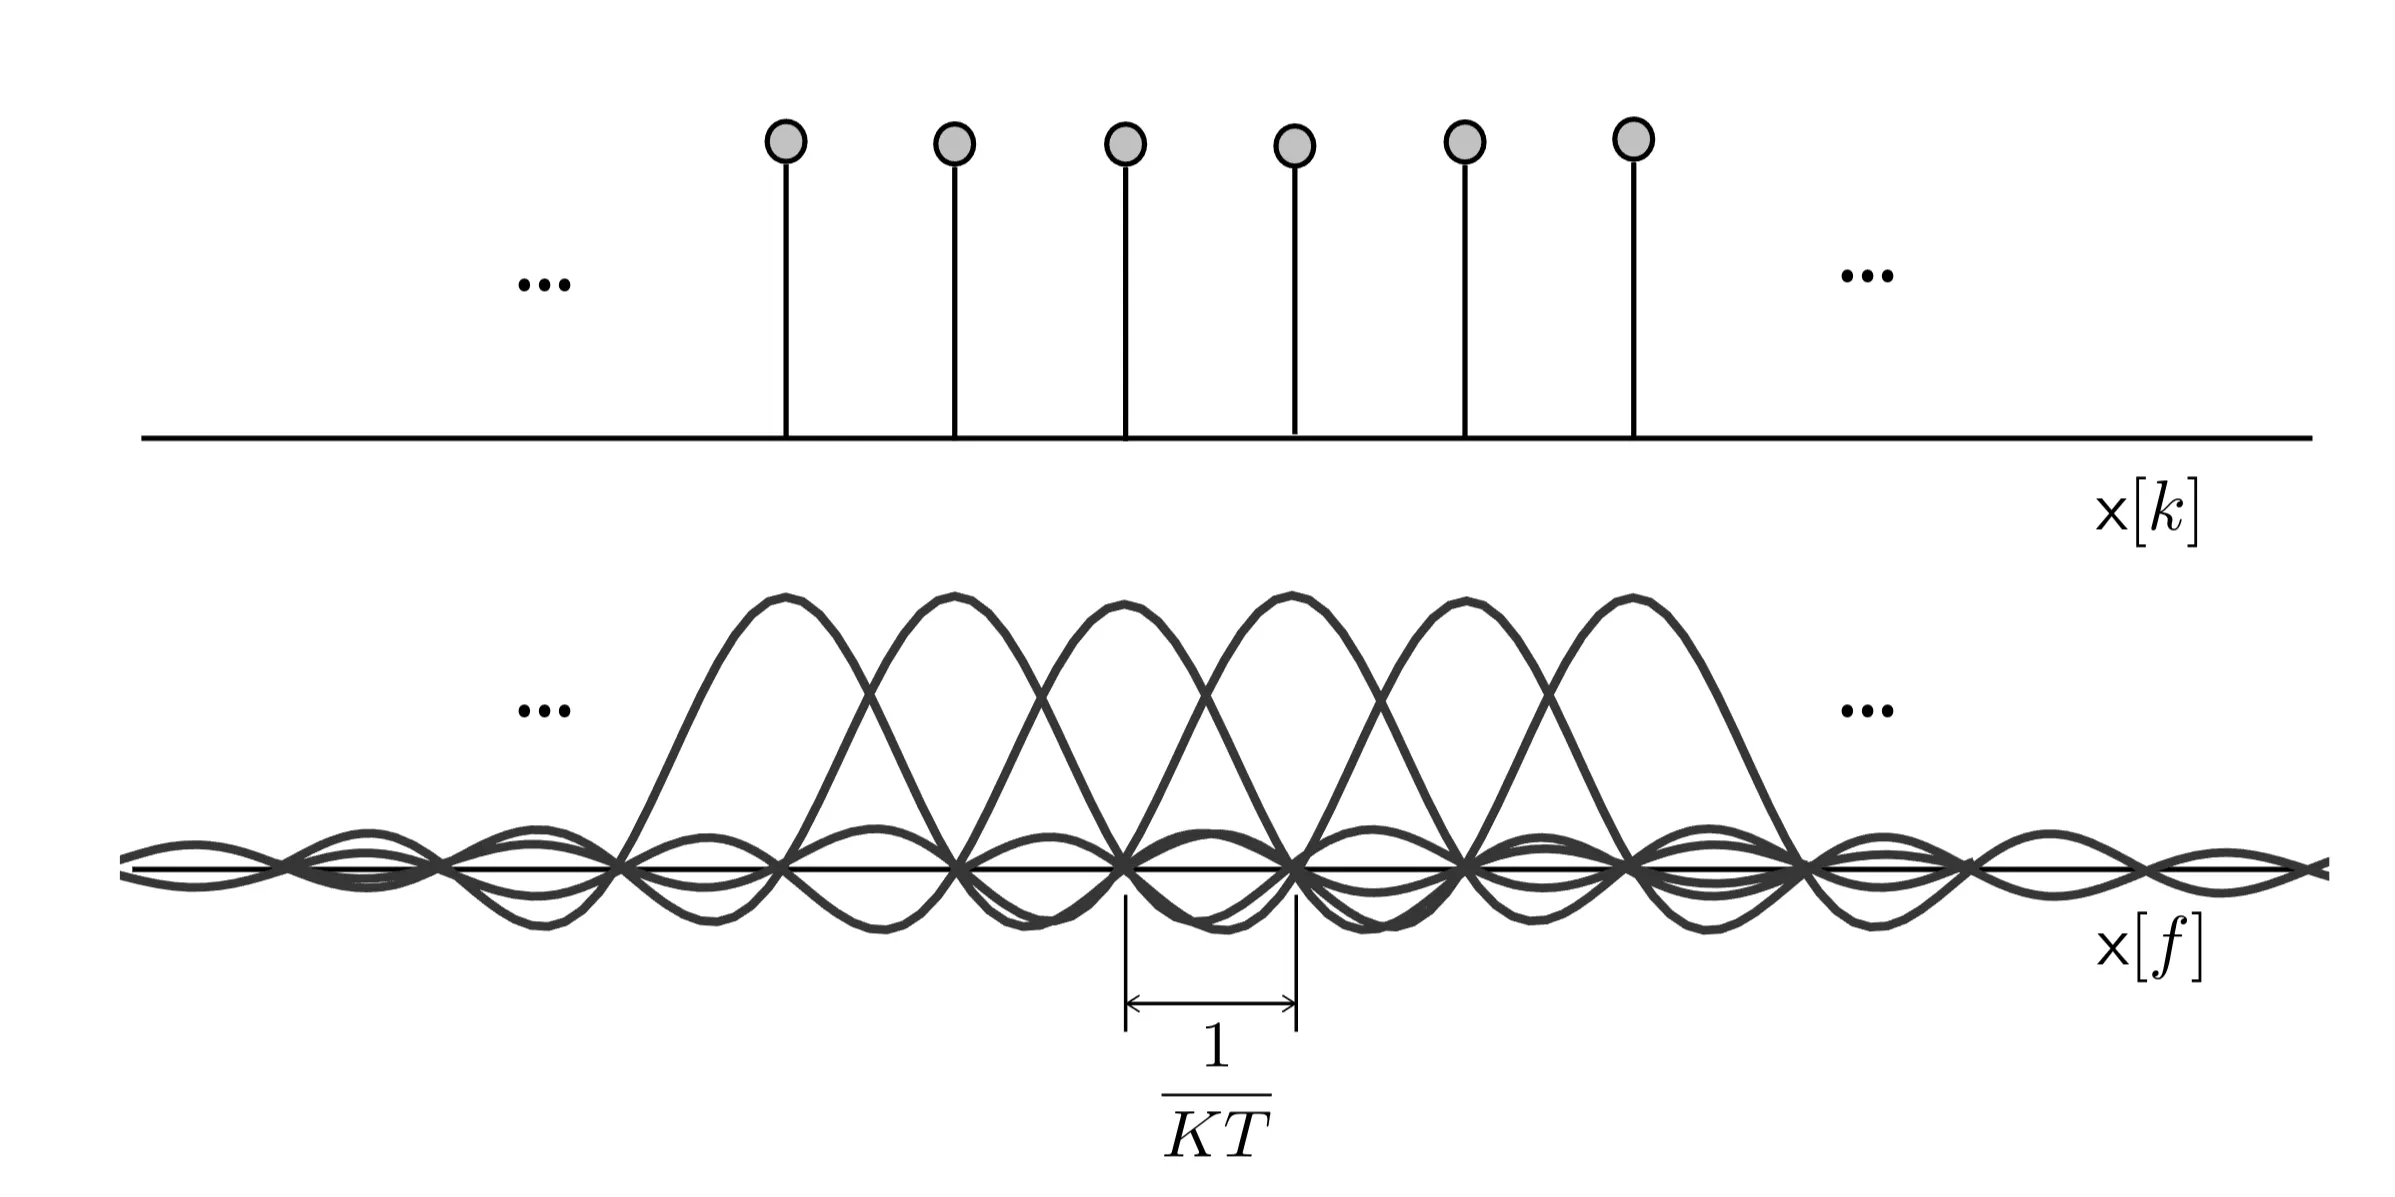
\includegraphics[width=0.6\textwidth]{Pictures/nome_immagine-006.png}
    \caption{Sinc functions in frequency domain spaced by 1/KT}
\end{figure}

\noindent
\colorbox{teal!10}{
    \begin{minipage}{\linewidth}
        \makebox[0pt][l]{\color{green}\rule[-6pt]{2pt}{20pt}} \hspace{10pt} This will allow for a perfect representation of our signal!
    \end{minipage}
}

Between OFDM symbols we have $KT$ seconds in time; if we consider them, the rect is $KT$ and the sinc in frequency will go to zero on the multiples of $1/KT$: this means that the carriers have no influence over each other whatsoever.

Edge subcarriers might be 0 (we'll see why shortly), leading to a \textbf{spectral efficiency penalty}.

Let's say we have a certain number of subcarriers:
\begin{figure}[h]
    \centering
    % Inserire qui l'immagine dei tre spettri (rosso, blu, nero)
    
\includegraphics[width=0.4\textwidth]{Pictures/image copy.png}
\end{figure}

We know that if our filter is a rect, it might interfere, cutting away a portion of the signals in the frequency domain:

\begin{figure}[h]
    \centering
    % Inserire qui l'immagine degli spettri con note verdi (256, 8, 8) e il filtro rect
    
\includegraphics[width=0.4\textwidth]{Pictures/image copy 2.png}
\end{figure}

We'd like to filter beforehand, but we can't generally do this; what we thus do is to \textbf{switch off the edge carriers} (in the example up here we switch off the first and last 8 edge carriers).
This means that the filter won't cut that sinc and it won't interfere with neighboring subcarriers.

In the following paragraph a more formal definition of penalty factor is given:

\vspace{0.5cm}

\noindent
\fcolorbox{cyan}{white}{
    \begin{minipage}{0.95\linewidth}
        \vspace{0.2cm}
        \textcolor{cyan}{\faPen\ \textbf{Penalty factor}}
        
        A completely separate but equally important definition is that of \textbf{penalty factor}: it is given by how much the usable bandwidth is in relation to the used bandwidth; the point is that in reality we'll always have some excess bandwidth which will go over our constraints: just to give an example, in \textit{example 2.23} the subcarrier spacing is $15 \mathrm{KHz}$ but it turns out that the actual subcarrier bandwidth is $\frac{500 \mathrm{MHz}}{300} = 16.66 \mathrm{KHz}$, more than what would be available. The penalty factor is thus calculated as
        
        \begin{align*}
            \text{Penalty factor} = \frac{\text{Usable bandwidth}}{\text{Used bandwidth}};
        \end{align*}
        
        this value is useful as whenever we have a channel of known spectral efficiency $R/B$ but we also know that we're exceeding the channel's bandwidth, we can correct the spectral efficiency as
        
        \begin{align*}
            (\text{Penalty factor}) \cdot \frac{R}{B}.
        \end{align*}
        
        Just as an extra piece of information, another way to see this is
        
        \begin{align*}
            \text{Penalty factor} = \frac{\text{Theoretically used bandwidth}}{\text{Actually used bandwidth}}.
        \end{align*}
        \vspace{0.1cm}
    \end{minipage}
}

\section[Examples of small exercises]{Examples of small exercises; many definitions of small values related to OFDM}

In the example we turn off the first and last 8 subcarriers for a system for which we have $K=256$: we'll have an \textbf{efficiency} which is limited:
\begin{align*}
    \frac{240}{256} < 1.
\end{align*}
We're thus having a total efficiency of
\begin{align*}
    \frac{256}{L+256} \cdot \frac{240}{256} < 1.
\end{align*}

We have some examples which \textbf{can also be conceived as some exam exercises} (as can be seen, they were indeed asked in the multiple-choices part of the exam).

\begin{itemize}[leftmargin=0pt, label={}]
    \item \textbf{Example 2.22} \\
    Let $T_{active} = 3.2 \, \mu\mathrm{s}$ with $K=256$ subcarriers and a cyclic prefix of length $L=64$.
    Find the chip period $T$, the passband bandwidth $1/T$, the subcarrier spacing, and the guard interval spanned by the cyclic prefix.
    
    \textit{Solution} \\
    The chip period $T$ satisfies $(256)T = 3.2 \, \mu\mathrm{s}$ and thus $T=12.5 \, \mathrm{ns}$. Then, $1/T = 80 \, \mathrm{MHz}$ and the subcarrier spacing is $\frac{1}{KT} = 312.5 \, \mathrm{kHz}$. The guard interval is $LT = 0.8 \, \mu\mathrm{s}$ and therefore channels with impulse responses of this duration can be handled.
    % Nota: I numeri nell'immagine originale sono molto sfuocati/illeggibili. Ho inserito i valori matematicamente coerenti con i dati forniti (3.2us / 256). 
    % Se l'immagine intendeva T_symbol = 3.2us (quindi (K+L)T), i numeri sarebbero diversi (T=10ns). 
    % Basandomi sulla sfocatura che sembra dire "10 ns" e "100 MHz", correggo sotto per fedeltà visiva seppur matematicamente ambiguo nel testo originale:
    
    \textit{[Alternative reading based on visual shape of blurry numbers]:} \\
    The chip period $T$ satisfies $(256+64)T = 3.2 \, \mu\mathrm{s}$ and thus $T = 10 \, \mathrm{ns}$. Then, $1/T = 100 \, \mathrm{MHz}$ and the subcarrier spacing is $\frac{1}{KT} = 390.6 \, \mathrm{kHz}$. The guard interval is $LT = 0.64 \, \mu\mathrm{s}$ and therefore channels with impulse responses of this duration can be handled.

    \item \textbf{Example 2.23} \\
    In LTE, the subcarrier spacing is $15 \, \mathrm{kHz}$ and every $5 \, \mathrm{MHz}$ of bandwidth accommodates $K=300$ subcarriers. What penalty factor should be applied to the spectral efficiency computed with $B=1/T$?
    
    \textit{Solution} \\
    Since $300 \cdot 15 \cdot 10^3 \, \mathrm{Hz}$ out of $5 \cdot 10^6 \, \mathrm{Hz}$ are used, the penalty factor equals $\frac{300 \cdot 15 \cdot 10^3}{5 \cdot 10^6} = 0.9$. \\
    For NR, this tightens up to $0.96$.
\end{itemize}

When the solution of the first says \textit{of this duration}, the actual correct thing is \textit{of this duration or less}!
In the second problem, the actual amount of carriers would be 333, but we use less so that we can avoid collision between external carriers.

\vspace{0.5cm}

\noindent
\fcolorbox{violet}{white}{
    \begin{minipage}{0.95\linewidth}
        \vspace{0.2cm}
        \textcolor{violet}{\faSkull \textbf{Guard interval}}
        
        The guard interval is the amount of time occupied by the cyclic prefix; it's called like this because it's an upper bound to how much our signal can be shifted while still being recoverable:
        
        \vspace{0.5em}
        \centering
        
\includegraphics[width=0.4\textwidth]{Pictures/image copy 3.png}
        \captionof*{figure}{The signal can still be reconstructed (blue arrows indicating $LT$ shift)}
        \vspace{0.1cm}
    \end{minipage}
}



\vspace{0.5cm}

\noindent
\fcolorbox{violet}{white}{
    \begin{minipage}{0.95\linewidth}
        \vspace{0.2cm}
        \textcolor{violet}{\faBook\ \textbf{Several definitions: $T, T_{OFDM}, \dots$}}
        
        Although we never did so in class, it seems necessary to introduce some values, with reference to the following figure (fig. 2.16):
        
        \begin{center}
            % Diagramma temporale OFDM: T, LT, T_OFDM, B, B/K
            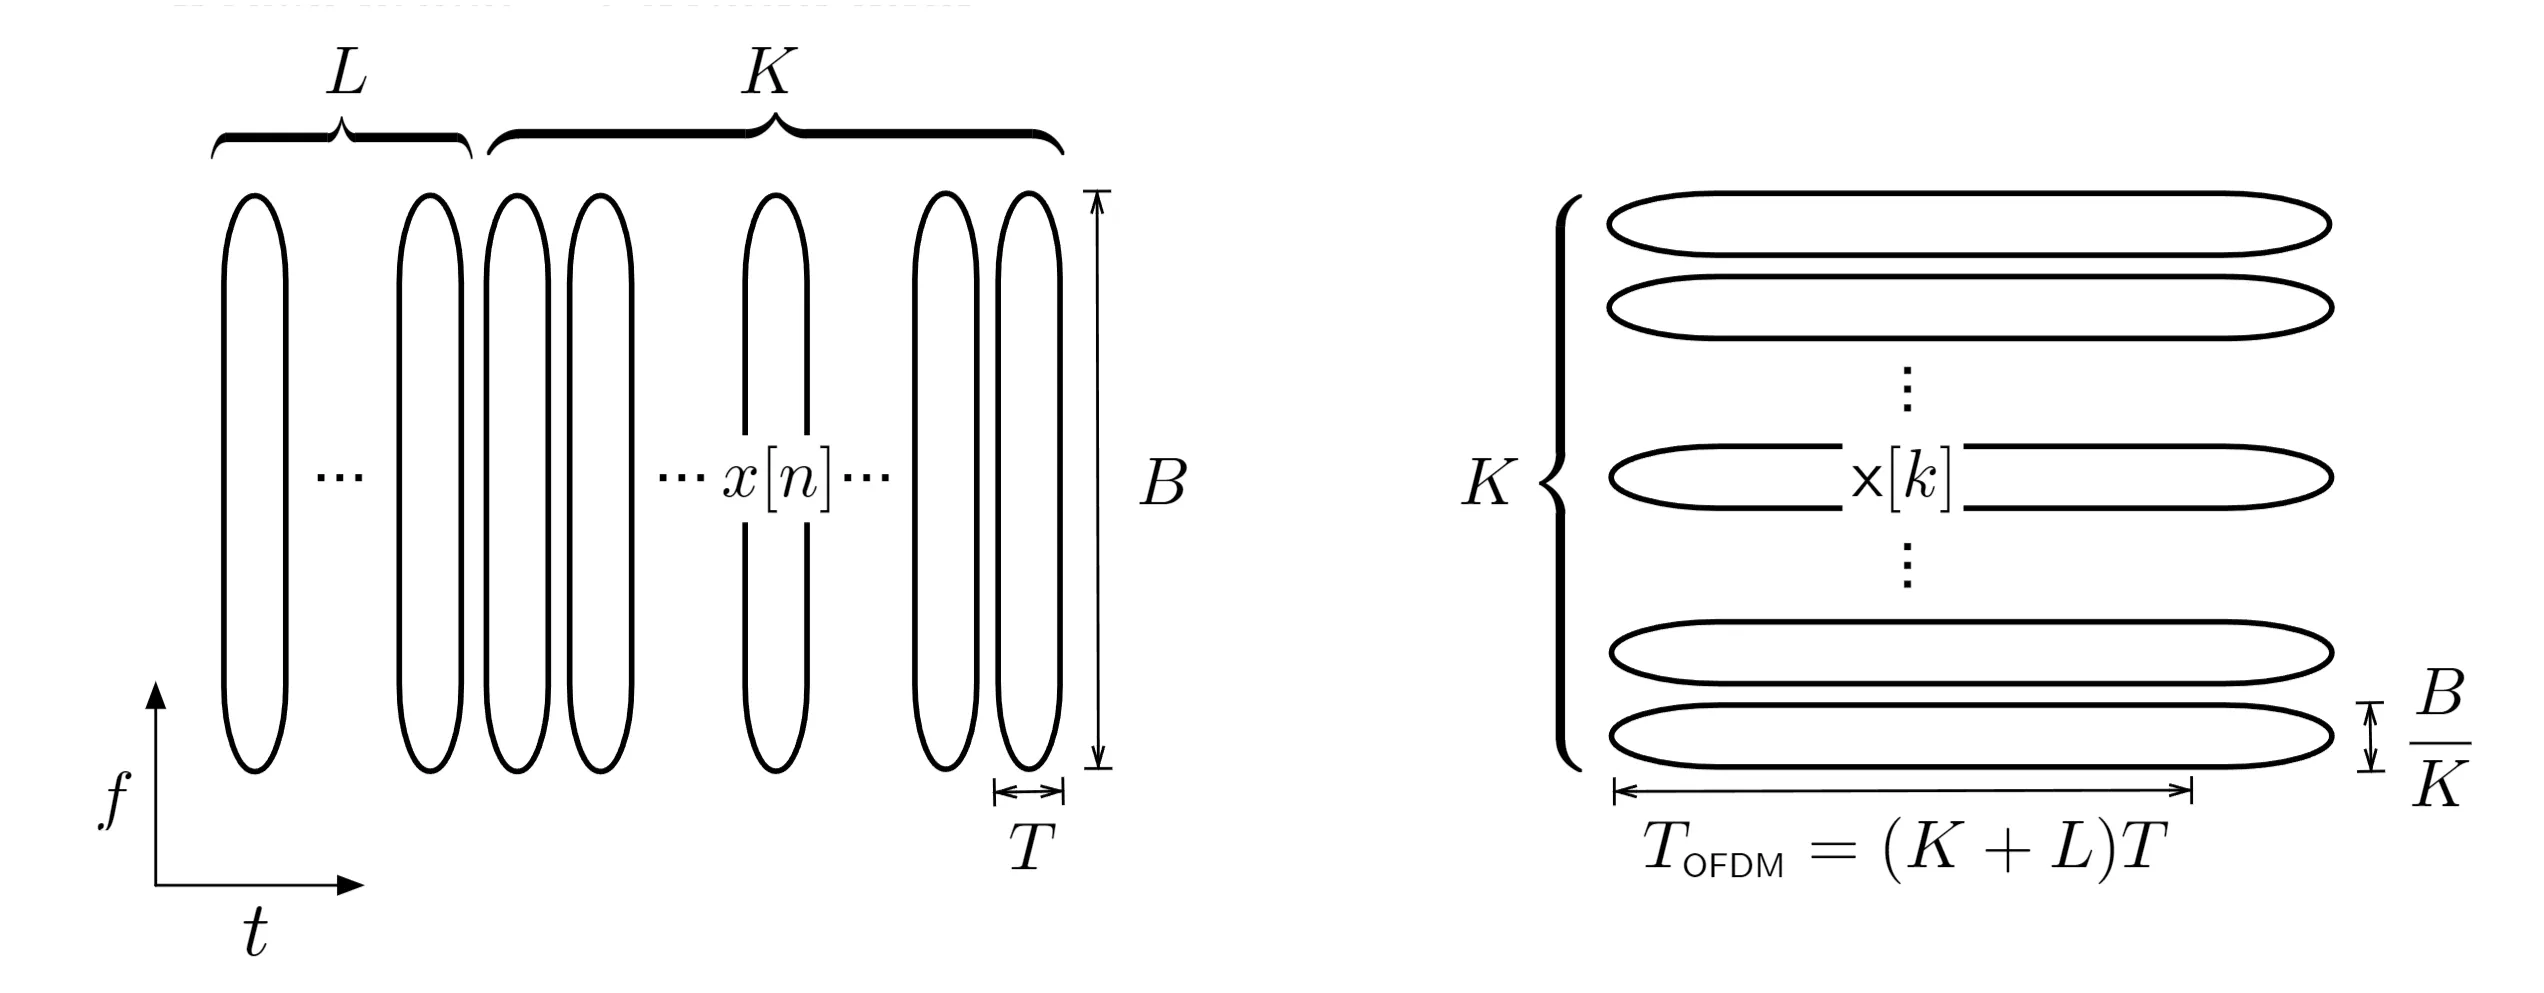
\includegraphics[width=0.7\textwidth]{Pictures/nome_immagine-008.png}
        \end{center}
        \begin{itemize}[label=\textbullet]
            \item $T$ is the \textbf{chip period}.
            \item $LT$ is the \textbf{guard interval}, as described above.
            \item $T_{OFDM}$ is the \textbf{period of a whole OFDM signal}, given by
            \[
            T_{OFDM} = (K+L)T.
            \]
            \item $B = 1/T$ is the \textbf{bandwidth} occupied by the \textbf{whole amount of subcarriers} collectively.
            \item $B/K = 1/KT$ is the \textbf{bandwidth occupied by a single subcarrier}; it also is the \textbf{subcarrier spacing}.
        \end{itemize}
        \vspace{0.1cm}
    \end{minipage}
}

\vspace{0.5cm}

\noindent
\fcolorbox{cyan}{white}{
    \begin{minipage}{0.95\linewidth}
        \vspace{0.2cm}
        \textcolor{cyan}{\faPen\ \textbf{Penalty factor}}
        
        A completely separate but equally important definition is that of \textbf{penalty factor}: it is given by how much the usable bandwidth is in relation to the used bandwidth; the point is that in reality we'll always have some excess bandwidth which will go over our constraints: just to give an example, in \textit{example 2.23} the subcarrier spacing is $15 \mathrm{kHz}$ but it turns out that the actual subcarrier bandwidth is $\frac{500 \mathrm{MHz}}{300} = 16.66 \mathrm{kHz}$, more than what would be available. The penalty factor is thus calculated as
        
        \begin{align*}
            \text{Penalty factor} = \frac{\text{Usable bandwidth}}{\text{Used bandwidth}};
        \end{align*}
        
        this value is useful as whenever we have a channel of known spectral efficiency $R/B$ but we also know that we're exceeding the channel's bandwidth, we can correct the spectral efficiency as
        
        \begin{align*}
            (\text{Penalty factor}) \cdot \frac{R}{B}.
        \end{align*}
        
        Just as an extra piece of information, another way to see this is
        
        \begin{align*}
            \text{Penalty factor} = \frac{\text{Theoretically used bandwidth}}{\text{Actually used bandwidth}}.
        \end{align*}
        \vspace{0.1cm}
    \end{minipage}
}

\vspace{1cm}

The same structure is found when extending this to MIMO-OFDM:

\begin{figure}[h]
    \centering
    % Inserire qui l'immagine degli spettri con note verdi (256, 8, 8) e il filtro rect
    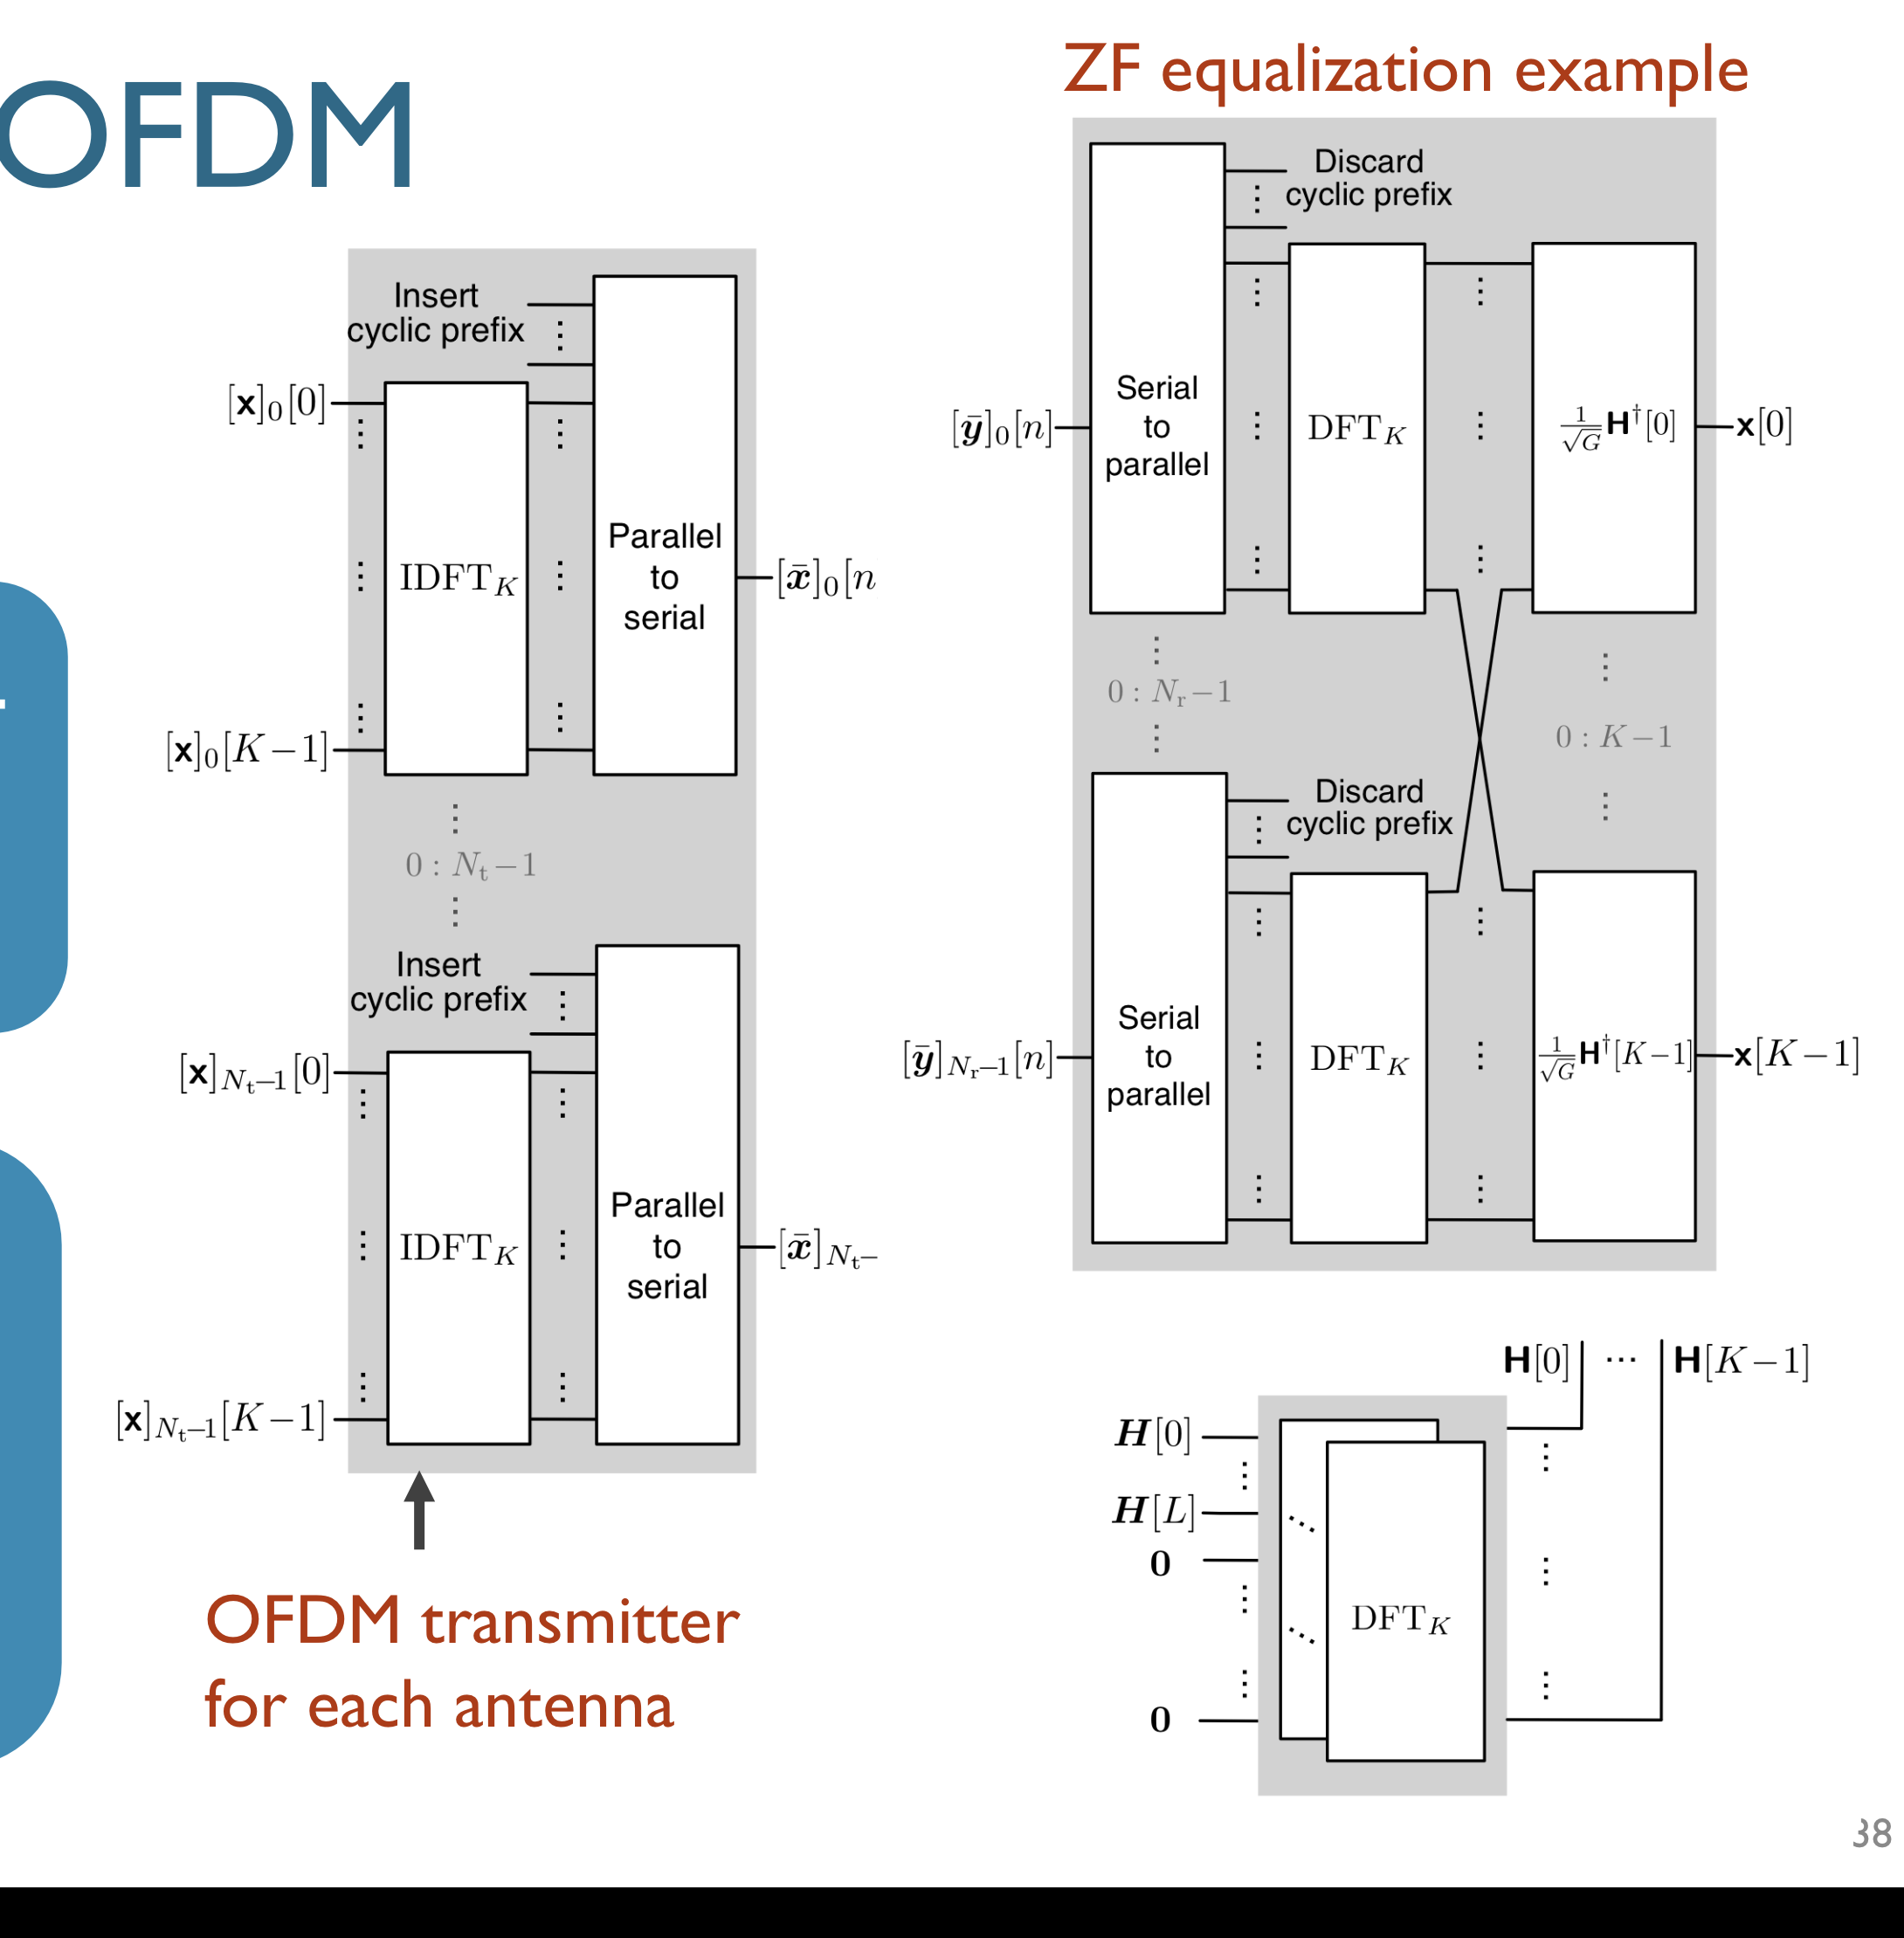
\includegraphics[width=0.4\textwidth]{Pictures/nome_immagine-009.png}
\end{figure}


All the IDFTs at the inputs of the different antennas are of the same sizes; we need the responses to be of the same sizes; $L$ must be the greatest of all channels and $K$ must be calculated knowing the penalty.

If we want to use as few resources as possible, we should customize $L, K$ for every antenna; we won't actually do this.


\end{document}